\documentclass{beamer}

\mode<presentation> {
%\usetheme{default}
%\usetheme{AnnArbor}
%\usetheme{Antibes}
%\usetheme{Bergen}
%\usetheme{Berkeley}
%\usetheme{Berlin}
%\usetheme{Boadilla}
%\usetheme{CambridgeUS}
%\usetheme{Copenhagen}
%\usetheme{Darmstadt}
%\usetheme{Dresden}
\usetheme{Frankfurt}
%\usetheme{Goettingen}
%\usetheme{Hannover}
%\usetheme{Ilmenau}
%\usetheme{JuanLesPins}
%\usetheme{Luebeck}
%\usetheme{Madrid}
%\usetheme{Malmoe}
%\usetheme{Marburg}
%\usetheme{Montpellier}
%\usetheme{PaloAlto}
%\usetheme{Pittsburgh}
%\usetheme{Rochester}
%\usetheme{Singapore}
%\usetheme{Szeged}
%\usetheme{Warsaw}

% As well as themes, the Beamer class has a number of color themes
% for any slide theme.
%\usecolortheme{albatross}
%\usecolortheme{beaver}
%\usecolortheme{beetle}
%\usecolortheme{crane}
%\usecolortheme{dolphin}
%\usecolortheme{dove}
%\usecolortheme{fly}
%\usecolortheme{lily}
\usecolortheme{orchid}
%\usecolortheme{rose}
%\usecolortheme{seagull}
%\usecolortheme{seahorse}
%\usecolortheme{whale}
%\usecolortheme{wolverine}

%\setbeamertemplate{footline} % To remove the footer line in all slides uncomment this line
%\setbeamertemplate{footline}[page number] % To replace the footer line in all slides with a simple slide count uncomment this line
%\setbeamertemplate{navigation symbols}{} % To remove the navigation symbols from the bottom of all slides uncomment this line
}

\usepackage{graphicx} % Allows including images
\usepackage{booktabs} % Allows the use of \toprule, \midrule and \bottomrule in tables
\usepackage[francais]{babel}
\usepackage[utf8]{inputenc}
\usepackage[T1]{fontenc}
\usepackage{transparent}
\usepackage{tikz}
\usepackage{tabularx}
\usepackage{hyperref}
\usepackage{fancyhdr}
\usepackage{float}
\usepackage{amssymb}
\usepackage{amsmath}
\usepackage[]{algorithm2e}
%\usepackage{media9}

\def\Put(#1, #2)#3{\leavevmode\makebox(0, 0){\put(#1, #2){#3}}}

\let\OLDtheorem=\theorem
\def\theorem{%
  \setbeamercolor{block title}{fg=white,bg=red!85!white}%
  \setbeamercolor{block body}{fg=black,bg=red!10!white}\OLDtheorem
}

\let\OLDdefinition=\definition
\def\definition{%
  \setbeamercolor{block title}{fg=white,bg=green!50!black}%
  \setbeamercolor{block body}{fg=black,bg=green!15!white}\OLDdefinition
}



%----------------------------------------------------------------------------------------
%	TITLE PAGE
%----------------------------------------------------------------------------------------

\title[Full title]{Une introduction à l'apprentissage automatique} % The short title appears at the bottom of every slide, the full title is only on the title page
%\subtitle{Lycée Gay-Lussac, Limoges}

\author{Eloïse BERTHIER}

\date{vendredi 8 mars 2019} 


\everymath{\displaystyle}

% show the table of contents before each section
\AtBeginSection[]
  {
    \ifnum \value{framenumber}>1
      \begin{frame}<beamer>
      \frametitle{Layout}
      \tableofcontents[currentsection]
      \end{frame}
    \else
    \fi
  }

\begin{document}

  \begin{frame}
  \titlepage 
  \Put(-20, 10){
\includegraphics[width=0.4\linewidth]{images/logo.jpg}}
\Put(230, 10){
\includegraphics[width=0.25\linewidth]{images/logo-ens.png}}

  \end{frame}
  
%\tableofcontents[sectionstyle=show/show, subsectionstyle=show/shaded/hide]
%  \tableofcontents[sectionstyle=show/show, subsectionstyle=hide]

% !TEX root=../main.tex



\begin{frame}{Introduction}

\vspace{-1em}


\Put(170, -140){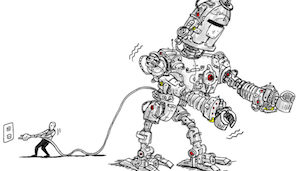
\includegraphics[width=0.45\linewidth]{images/robot.jpg}}

\end{frame}

\begin{frame}{Une histoire d'algorithmes}

Peut-on trouver un algorithme pour :
\begin{itemize}
\item faire cuire des pâtes ?
\item trouver son chemin dans une ville ?
\item trouver un chat dans une image ? 
\item gagner une partie d'échecs ?
\end{itemize}

\end{frame}

\begin{frame}{La régression}

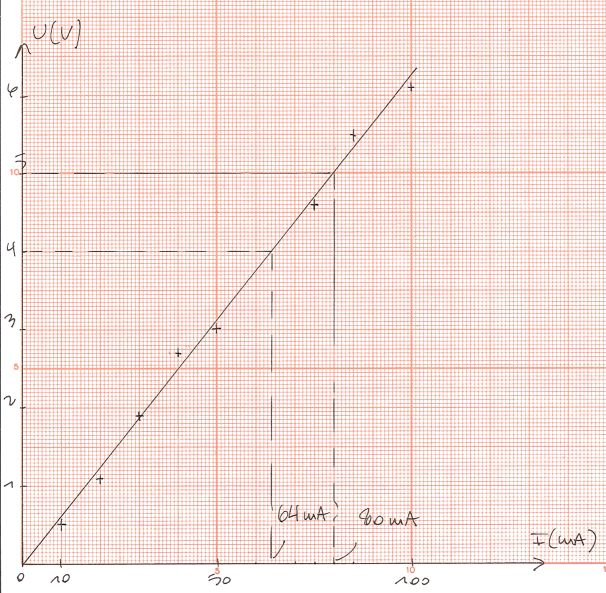
\includegraphics[width=7cm]{images/droite.jpg}
\end{frame}


\begin{frame}{La souris, le fromage et le poison\footnote{{\scriptsize Vincent Lepetit, \textit{Deep Learning} (MVA, CentraleSupelec)}}}

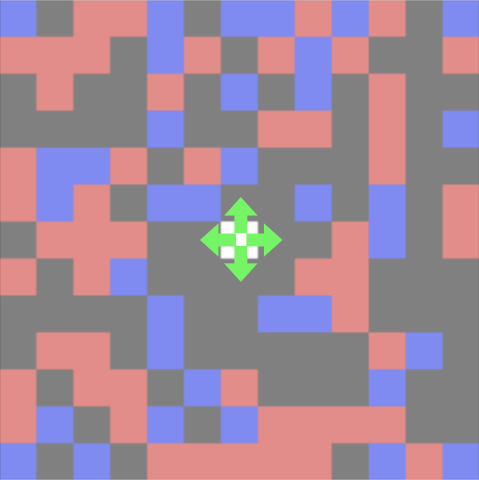
\includegraphics[width=5cm]{images/board.jpeg} 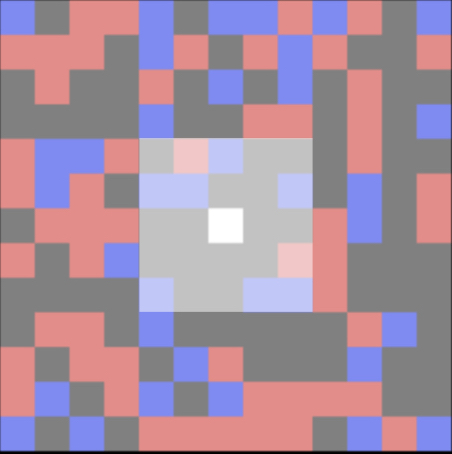
\includegraphics[width=5cm]{images/visu.jpeg}

Récompense +1 si la souris passe par une case rouge (fromage)

Pénalité -1 si la souris passe par une case bleue (poison)

\end{frame}

\begin{frame}

Que remarque-t-on ?

\begin{itemize}
\item l'ordinateur a appris
\item mais bien plus lentement qu'un humain ou même une souris !
\item on aurait pu trouver un algorithme très simple
\item et si on ne connait pas la réponse à l'avance ? (cf Go)
\end{itemize}

\end{frame}



%\begin{frame}[allowframebreaks]
  %      \frametitle{References}
    %    \bibliographystyle{amsalpha}
      %  \bibliography{biblio.bib}
%\end{frame}


\end{document}
